\documentclass[conference]{IEEEtran}
% ---- shared preamble material (included by paper.tex and report.tex) ----
\usepackage{amsmath,amssymb,booktabs,siunitx,xcolor,multirow,graphicx}
\usepackage{pgfplots,pgfplotstable}
\usepackage{tikz}
\usetikzlibrary{positioning,arrows.meta,fit,calc}
\pgfplotsset{compat=1.16}
\newif\ifillustrative \illustrativefalse  % data/*.csv are generated by sim/analyze.py from results/
% Generated by sim/analyze.py. Do not edit.
\newcommand{\hOneAdaptSlope}{0.628} % results/burst.jsonl (fit)
\newcommand{\hOneCapSlope}{0.00232} % results/burst.jsonl (fit)
\newcommand{\hOneFpSlope}{5.92} % results/burst.jsonl (fit)
\newcommand{\hOneRrSlope}{6} % results/burst.jsonl (fit)
\newcommand{\kneeFps}{92.1} % results/fps.jsonl (drop rate crosses 1%)
\newcommand{\kneePredFps}{160} % results/predictions.json
\newcommand{\policyFps}{120} % results/policy.jsonl
\newcommand{\predCAPBound}{0.72} % results/burst.jsonl, predictions.json
\newcommand{\predCAPMax}{2.39} % results/burst.jsonl, predictions.json
\newcommand{\predCAPP99}{1.42} % results/burst.jsonl, predictions.json
\newcommand{\predFPBound}{5.2} % results/burst.jsonl, predictions.json
\newcommand{\predFPMax}{8.17} % results/burst.jsonl, predictions.json
\newcommand{\predFPP99}{7.11} % results/burst.jsonl, predictions.json
\newcommand{\predRRBound}{10.3} % results/burst.jsonl, predictions.json
\newcommand{\predRRMax}{12.1} % results/burst.jsonl, predictions.json
\newcommand{\predRRP99}{10.8} % results/burst.jsonl, predictions.json
  % every number in the text; each macro names its source
\newcommand{\tbd}[1][X]{\textcolor{red}{[#1]}}
\newcommand{\illusnote}{\ifillustrative\\[-2pt]\textcolor{red}{\scriptsize ILLUSTRATIVE SHAPE, NOT RESULTS: replace data/*.csv}\fi}
\newcommand{\imu}{\textsc{imu}}
\newcommand{\cam}{\textsc{cam}}
\newcommand{\npu}{\textsc{npu}}
\newcommand{\pone}{\ensuremath{p_{99}}}
\pgfplotsset{dmaplot/.style={width=\linewidth,height=0.72\linewidth,grid=major,
  grid style={gray!25},tick label style={font=\scriptsize},label style={font=\footnotesize},
  legend style={font=\tiny,at={(0.02,0.98)},anchor=north west},every axis plot/.append style={thick,mark size=1.6pt}}}

\begin{document}
\title{Smarter Buses or Fewer Frames? Burst Sizing, Arbitration and Frame Dropping on a Drone SoC}
\author{\IEEEauthorblockN{Ahad Ulla Baig}\IEEEauthorblockA{Dept. of Artificial Intelligence\\and Machine Learning\\Ramaiah Institute of Technology\\Bengaluru, India\\ ahadullabaig.16@gmail.com}\and \IEEEauthorblockN{Divisha Gera}\IEEEauthorblockA{Dept. of Artificial Intelligence\\and Machine Learning\\Ramaiah Institute of Technology\\Bengaluru, India\\ divisha.018@gmail.com}\and \IEEEauthorblockN{Charithra G}\IEEEauthorblockA{Dept. of Artificial Intelligence\\and Machine Learning\\Ramaiah Institute of Technology\\Bengaluru, India\\ charithra754@gmail.com}}
\maketitle

\begin{abstract}
A drone SoC shares one memory path between a camera DMA engine, a high-rate IMU/telemetry master and an inference core. Large camera bursts can block small IMU packets, so the usual fixes are to drop frames, cap bursts, or schedule with ages and deadlines. We built a deterministic event-driven simulator of this SoC and ask when scheduling beats simply dropping frames at equal bandwidth and energy. We state three falsifiable hypotheses, predict results with an analytic bound before running the simulator, and log the cause of every stall. At the saturation knee of \tbd[X] fps, the IMU \pone{} latency is \tbd[X]~$\mu$s under fixed priority with 1~KB bursts, \tbd[X]~$\mu$s with burst capping, and \tbd[X]~$\mu$s when frames are dropped. Traffic is driven by frame-change intensity from ERA/CapERA aerial clips and a logged IMU stream. \tbd[Replace with the final one-sentence verdict, including any setting where plain frame dropping matches or beats scheduling.]
\end{abstract}
\begin{IEEEkeywords}
DMA, bus arbitration, memory contention, burst size, drone SoC, frame dropping, DVFS
\end{IEEEkeywords}

\section{Introduction}
Onboard perception on a small drone must share one memory system among traffic classes with very different needs. The camera moves megabytes per frame in long bursts. The IMU sends tens of bytes at hundreds of hertz and feeds a control loop that cannot tolerate a late sample. The inference core reads frame tiles and writes features. When these collide, a long non-preemptive burst can delay a tiny packet by the whole burst time.

Two cheap remedies need no new hardware policy: drop frames when queues back up, or fix a larger (or smaller) burst. Scheduling policies such as burst splitting or age-aware arbitration promise more, but they add logic, and their benefit may vanish once total bandwidth and energy are held equal. We follow the equal-budget method of~\cite{baig2026fewer}, which compared a gated kernel with simply running a model less often.

\textbf{Hypotheses.} Each can be refuted by the experiments in Section~\ref{sec:results}.
\begin{itemize}
\item \textbf{H1 (burst blocking).} IMU \pone{} latency grows linearly with the camera burst size under fixed-priority and round-robin arbitration, and is bounded by the cap under burst capping.
\item \textbf{H2 (equal budget).} At equal average DRAM bandwidth and energy, adaptive burst splitting lowers IMU \pone{} latency without raising frame age relative to frame dropping.
\item \textbf{H3 (when dropping wins).} Above the saturation knee, where $\rho\!\ge\!1$, scheduling cannot restore freshness and frame dropping gives equal or lower frame age.
\end{itemize}

\textbf{Contributions.}
\begin{itemize}
\item A deterministic event-driven SoC simulator with per-request stall attribution (arbitration, burst blocking, cache, DRAM saturation).
\item An analytic latency bound written before simulation, and a comparison of predicted against simulated values.
\item An equal-budget comparison of frame dropping, fixed bursts, burst capping and age/deadline-aware scheduling, with traces derived from real aerial video.
\end{itemize}

\section{Background and Related Work}
\textbf{Memory scheduling.} DRAM-aware schedulers reorder requests to raise row-buffer hits~\cite{rixner2000}, and fairness-oriented ones bound slowdown across cores~\cite{mutlu2007,kim2010atlas}. Bandwidth regulation isolates masters by budgeting accesses per period~\cite{yun2013memguard}, and predictable controllers give worst-case latency bounds~\cite{akesson2007predator}. Our burst cap is a simple regulator of this kind applied at the DMA.\\
\textbf{Simulation.} Full-system and DRAM simulators exist~\cite{binkert2011gem5,kim2016ramulator}. We use a purpose-built simulator so that every stall cycle has a recorded cause.\\
\textbf{Workloads.} ERA~\cite{mou2020era} and CapERA~\cite{bashmal2023capera} supply aerial video whose frame-change intensity shapes the traffic.

\section{System and Workload Model}
\subsection{Architecture}
Fig.~\ref{fig:arch} shows the modelled SoC. Three masters (camera DMA, IMU/telemetry, NPU/CPU) share one bus. The NPU has private L1/L2 caches with a finite number of MSHRs, and a shared cache or scratchpad sits in front of the memory controller. The bus is non-preemptive: once a burst is granted it holds the bus for its whole duration.
\begin{figure}[t]\centering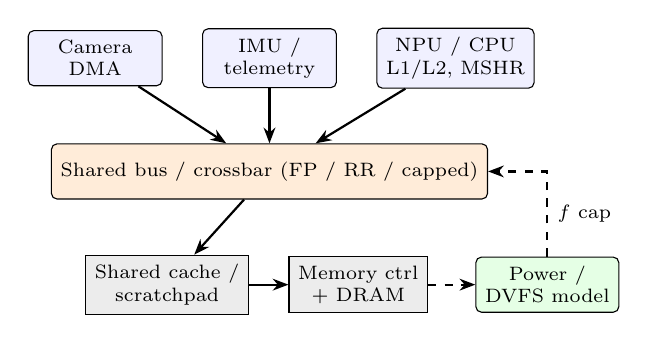
\begin{tikzpicture}[font=\scriptsize,node distance=5mm,
 blk/.style={draw,rounded corners=2pt,minimum height=7mm,minimum width=17mm,align=center,fill=blue!6},
 mem/.style={draw,minimum height=7mm,minimum width=17mm,align=center,fill=gray!15},
 ar/.style={-{Stealth[length=2mm]},thick}]
 \node[blk] (cam) {Camera\\DMA};
 \node[blk,right=of cam] (imu) {IMU /\\telemetry};
 \node[blk,right=of imu] (npu) {NPU / CPU\\L1/L2, MSHR};
 \node[blk,fill=orange!15,below=7mm of imu,minimum width=48mm] (bus) {Shared bus / crossbar (FP / RR / capped)};
 \node[mem,below=7mm of bus,xshift=-13mm] (llc) {Shared cache /\\scratchpad};
 \node[mem,right=of llc] (dram) {Memory ctrl\\+ DRAM};
 \node[blk,fill=green!10,right=6mm of dram,minimum width=17mm] (pw) {Power /\\DVFS model};
 \draw[ar] (cam)--(bus); \draw[ar] (imu)--(bus); \draw[ar] (npu)--(bus);
 \draw[ar] (bus)--(llc); \draw[ar] (llc)--(dram); \draw[ar,dashed] (dram)--(pw);
 \draw[ar,dashed] (pw.north) |- node[pos=0.25,right]{$f$ cap} (bus.east);
\end{tikzpicture}
\caption{Modelled drone SoC. Dashed arrows: the power model measures traffic and caps the clock $f$.}\label{fig:arch}\end{figure}

\subsection{Traffic and utilisation}
Camera demand is $D_c=\phi F$ for frame rate $\phi$ and frame size $F$ bytes. IMU demand is $D_i=\lambda_i S_i$ for rate $\lambda_i$ and packet size $S_i$. The NPU reads a fraction $\gamma$ of each processed frame. With a bus of peak rate $BW$ and burst efficiency $\eta(B)$, the utilisation is
\begin{equation}
\rho=\frac{D_c+D_i+D_n}{BW\,\eta(B)},\qquad \eta(B)=\frac{B}{B+B_o},
\label{eq:rho}
\end{equation}
where $B_o$ is the per-burst overhead expressed in bytes of lost bus time (arbitration and row activation). The saturation knee is the frame rate at which $\rho=1$.

\subsection{Predicted blocking latency}
For one burst in flight and arbitration time $t_a$, the worst-case IMU wait is
\begin{align}
W^{\mathrm{FP}}_{i}&\le t_a+\frac{B_{\max}}{BW},\label{eq:fp}\\
W^{\mathrm{RR}}_{i}&\le t_a+\frac{(N-1)\,B_{\max}}{BW},\label{eq:rr}\\
W^{\mathrm{cap}}_{i}&\le t_a+\frac{B_{\mathrm{cap}}}{BW},\quad B_{\max}\rightarrow\min(B_{\max},B_{\mathrm{cap}}),\label{eq:cap}
\end{align}
with $N$ masters. Smaller bursts cost bandwidth through $\eta(B)$, so the camera frame time grows to $T_c=\lceil F/B_{\mathrm{cap}}\rceil (B_{\mathrm{cap}}+B_o)/BW$. Eqs.~(\ref{eq:fp})--(\ref{eq:cap}) are bounds on a single wait; they ignore queueing and are therefore predictions of the tail to be checked against the simulator, not guarantees.

\subsection{Freshness, power and the equal-budget rule}
Frame age at inference is $A_k=t^{\mathrm{done}}_k-t^{\mathrm{cap}}_k$ for frame $k$, and a frame is dropped if its input queue holds more than $Q$ frames. Power follows
\begin{align}
P&=P_s+\alpha C V^2 f+e_b\,r_{\mathrm{DRAM}},\label{eq:power}\\
f&=\max\{f'\le f_{\max}: P(f')\le P_{\mathrm{cap}}\},\label{eq:dvfs}
\end{align}
with static power $P_s$, activity $\alpha$, switched capacitance $C$, DRAM energy per byte $e_b$ and DRAM rate $r_{\mathrm{DRAM}}$. Energy per processed frame is $E=\int P\,dt/N_{\mathrm{proc}}$. Policies are compared only when
\begin{equation}
\Big|\bar r_{\mathrm{DRAM}}^{\,\pi}-\bar r_{\mathrm{DRAM}}^{\,\mathrm{drop}}\Big|\le\epsilon_{b},\qquad \Big|E^{\pi}-E^{\mathrm{drop}}\Big|\le\epsilon_{e},
\label{eq:equal}
\end{equation}
where frame dropping matches a target budget by dropping a fraction $\delta$ of frames, so $D_c\rightarrow(1-\delta)D_c$.

\section{Scheduling Policies}
\textbf{Baselines.} \emph{Frame dropping}: skip a frame when the input queue exceeds $Q$. \emph{Fixed burst}: camera burst $B_c$ is constant, with fixed priority ($\imu>\npu>\cam$) or round-robin.\\
\textbf{Proposed.} \emph{Burst capping} limits every master to $B_{\mathrm{cap}}$. \emph{Adaptive splitting} splits a camera burst into pieces of size $B_s$ whenever an IMU packet is pending. \emph{Age/deadline-aware} arbitration grants the request with the smallest slack
\begin{equation}
s_j=d_j-(t-t_j^{\mathrm{arr}})-\frac{B_j}{BW},
\end{equation}
where $d_j$ is the request's deadline (IMU: its control-loop period; camera: the frame deadline).

\section{Experimental Setup}
\subsection{Simulator}
The simulator is deterministic and event-driven, with events \texttt{IMU\_ARRIVAL}, \texttt{CAM\_FRAME\_START}, \texttt{DMA\_BURST\_REQ}, \texttt{BUS\_GRANT}, \texttt{CACHE\_HIT/MISS}, \texttt{DRAM\_SERVICE} and \texttt{COMPUTE\_TILE\_DONE}. Each request records its stall by cause, so that
\begin{equation}
T^{\mathrm{stall}}_j=T^{\mathrm{arb}}_j+T^{\mathrm{burst}}_j+T^{\mathrm{cache}}_j+T^{\mathrm{dram}}_j.
\end{equation}
Table~\ref{tab:params} lists the parameters. Runs use fixed seeds and a warm-up before measuring; every table and figure is regenerated from committed CSV files.
\begin{table}[t]\centering\caption{Default simulator parameters (assumed configuration, swept where noted).}\label{tab:params}
\small\begin{tabular}{@{}ll@{}}\toprule
Parameter & Value\\\midrule
DRAM peak bandwidth $BW$ & \tbd[12.8] GB/s\\
Camera rate $\phi$ / frame $F$ & 30--120 fps (swept) / \tbd[0.6] MB\\
Camera burst $B_c$ & 64 B -- 2 KB (swept)\\
IMU rate / packet $S_i$ & 200--1000 Hz / \tbd[32] B\\
Cache (size, ways, policy) & \tbd[256 KB, 8, write-back]\\
MSHRs & \tbd[8]\\
$P_{\mathrm{cap}}$, $f_{\max}$ & \tbd[X] W, \tbd[X] MHz\\
Queue limit $Q$ & \tbd[2] frames\\\bottomrule
\end{tabular}\end{table}

\subsection{Traces}
\emph{Synthetic stress traces} sweep frame rate, frame size, burst length and background traffic to locate the knee. \emph{Aerial traces} take per-frame change intensity from ERA/CapERA clips~\cite{mou2020era,bashmal2023capera}; the NPU's tile reads scale with that intensity, and the IMU stream is a logged or synthetic telemetry trace with bursts at manoeuvres. We report the number of clips and their motion groups: \tbd[N clips].

\subsection{Metrics and statistics}
We report IMU \pone{} and maximum latency, frame-to-inference age, drop rate, DRAM utilisation, bus idle and stall cycles, cache miss rate, MSHR occupancy and energy. Intervals are 95\% bootstrap intervals over \tbd[N] seeds or clips. A policy ``wins'' only if its interval excludes the baseline's at equal budget (Eq.~\ref{eq:equal}).

\section{Results and Discussion}\label{sec:results}
\subsection{Predicted against simulated}
Table~\ref{tab:pred} compares Eqs.~(\ref{eq:fp})--(\ref{eq:cap}) with the simulator. \tbd[State where the bound holds, where queueing breaks it, and by how much.]
\begin{table}[t]\centering\caption{IMU wait at $B_c=1$~KB, 60~fps: bound against simulated.}\label{tab:pred}
\small\begin{tabular}{@{}lrrr@{}}\toprule
Policy & Bound ($\mu$s) & Sim.\ \pone{} & Sim.\ max\\\midrule
Fixed priority & \tbd & \tbd & \tbd\\
Round-robin & \tbd & \tbd & \tbd\\
Burst-capped & \tbd & \tbd & \tbd\\\bottomrule
\end{tabular}\end{table}

\subsection{H1: burst blocking}
\begin{figure}[t]\centering\begin{tikzpicture}\begin{axis}[dmaplot,xmode=log,log basis x=2,xlabel={Camera DMA burst $B_{c}$ (bytes)},
 ylabel={IMU \pone{} latency ($\mu$s)},xtick={64,128,256,512,1024,2048},xticklabels={64,128,256,512,1K,2K}]
\addplot table[col sep=comma,x=burst,y=fp]{data/burst.csv};\addlegendentry{Fixed prio.}
\addplot table[col sep=comma,x=burst,y=rr]{data/burst.csv};\addlegendentry{Round-robin}
\addplot table[col sep=comma,x=burst,y=cap]{data/burst.csv};\addlegendentry{Burst-capped}
\addplot table[col sep=comma,x=burst,y=adapt]{data/burst.csv};\addlegendentry{Adaptive split}
\end{axis}\end{tikzpicture}\illusnote
\caption{IMU \pone{} latency against camera burst size at 60~fps.}\label{fig:burst}\end{figure}
Fig.~\ref{fig:burst} sweeps $B_c$. \tbd[Fit slope against $1/BW$ of Eq.~(\ref{eq:fp}); report whether H1 holds.]

\subsection{Saturation knee}
\begin{figure}[t]\centering\begin{tikzpicture}\begin{axis}[dmaplot,xlabel={Camera frame rate (fps)},ylabel={Utilisation $\rho$ / drop rate},
 ymin=0,ymax=1.05,legend style={at={(0.02,0.98)},anchor=north west}]
\addplot[blue,mark=*] table[col sep=comma,x=fps,y=rho]{data/knee.csv};\addlegendentry{$\rho$, power-capped}
\addplot[blue,dashed,mark=o] table[col sep=comma,x=fps,y=rho_pinned]{data/knee.csv};\addlegendentry{$\rho$, clock pinned}
\addplot[red,mark=square*] table[col sep=comma,x=fps,y=drop]{data/knee.csv};\addlegendentry{drop rate, power-capped}
\addplot[red,dashed,mark=square] table[col sep=comma,x=fps,y=drop_pinned]{data/knee.csv};\addlegendentry{drop rate, clock pinned}
\end{axis}\end{tikzpicture}\illusnote
\caption{Bus utilisation $\rho$ (Eq.~\ref{eq:rho}) against camera frame rate.}\label{fig:knee}\end{figure}
Fig.~\ref{fig:knee} locates the knee at \tbd[X] fps. Beyond it, queues grow without bound unless frames are dropped.

\subsection{H2 and H3: equal-budget comparison}
\begin{figure}[t]\centering\begin{tikzpicture}\begin{axis}[dmaplot,xlabel={Frame drop rate (\%)},ylabel={Mean frame age at inference (ms)},
 legend style={at={(0.98,0.98)},anchor=north east}]
\addplot table[col sep=comma,x=drop,y=age]{data/policy_drop.csv};\addlegendentry{Frame dropping}
\addplot table[col sep=comma,x=drop,y=age]{data/policy_adapt.csv};\addlegendentry{Adaptive burst}
\addplot table[col sep=comma,x=drop,y=age]{data/policy_edf.csv};\addlegendentry{Age/deadline-aware}
\end{axis}\end{tikzpicture}\illusnote
\caption{Frame age against drop rate at equal DRAM bandwidth and energy (Eq.~\ref{eq:equal}).}\label{fig:policy}\end{figure}
\begin{table}[t]\centering\caption{Equal-budget comparison at \tbd[X] fps (mean $\pm$ 95\% CI).}\label{tab:policy}
\small\begin{tabular}{@{}lrrrr@{}}\toprule
Policy & IMU \pone{} ($\mu$s) & Age (ms) & Drop (\%) & $E$ (mJ)\\\midrule
Frame dropping & \tbd & \tbd & \tbd & \tbd\\
Fixed 1 KB, FP & \tbd & \tbd & \tbd & \tbd\\
Burst-capped & \tbd & \tbd & \tbd & \tbd\\
Adaptive split & \tbd & \tbd & \tbd & \tbd\\
Age/deadline & \tbd & \tbd & \tbd & \tbd\\\bottomrule
\end{tabular}\end{table}
Fig.~\ref{fig:policy} and Table~\ref{tab:policy} test H2 and H3. \tbd[Say which policies win, which tie, and where dropping wins.]

\subsection{Where the stalls go}
\begin{figure}[t]\centering\begin{tikzpicture}\begin{axis}[dmaplot,ybar stacked,bar width=11pt,ymin=0,ymax=100,ylabel={Share of stall cycles (\%)},
 symbolic x coords={FP,RR,Capped,Adaptive},xtick=data,legend style={at={(0.5,-0.18)},anchor=north,legend columns=2}]
\addplot[fill=blue!50] table[col sep=comma,x=policy,y=arb]{data/stall.csv};\addlegendentry{Arbitration wait}
\addplot[fill=orange!70] table[col sep=comma,x=policy,y=burst]{data/stall.csv};\addlegendentry{Burst blocking}
\addplot[fill=green!50!black] table[col sep=comma,x=policy,y=cache]{data/stall.csv};\addlegendentry{Cache miss}
\addplot[fill=gray!60] table[col sep=comma,x=policy,y=dram]{data/stall.csv};\addlegendentry{DRAM saturation}
\end{axis}\end{tikzpicture}\illusnote
\caption{Stall-cycle share by cause for each policy.}\label{fig:stall}\end{figure}
Fig.~\ref{fig:stall} separates blocking from saturation. A policy that shortens blocking but leaves DRAM saturation unchanged only moves the stall. \tbd[Interpret.]

\subsection{Energy and clocks}
\begin{figure}[t]\centering\begin{tikzpicture}\begin{axis}[dmaplot,xlabel={Policy},ylabel={Energy per processed frame (mJ)},
 ybar,bar width=12pt,symbolic x coords={Drop,FP,RR,Capped,Adaptive},xtick=data,ymin=0]
\addplot[fill=teal!50] table[col sep=comma,x=policy,y=energy]{data/energy.csv};
\end{axis}\end{tikzpicture}\illusnote
\caption{Energy per processed frame at equal bandwidth.}\label{fig:energy}\end{figure}
Fig.~\ref{fig:energy} tests whether smarter scheduling saves energy or only shifts work, and whether the power cap in Eq.~(\ref{eq:power}) changes the sustained clock. \tbd[Interpret.]

\section{Limitations}
Results come from a simulator, not silicon. DRAM timing is simplified to \tbd[model], and the power model uses assumed coefficients. The bound in Eqs.~(\ref{eq:fp})--(\ref{eq:cap}) ignores queueing. Aerial traces set traffic intensity only; they do not exercise a real image pipeline. \tbd[Add any further threats found while running.]

\section{Conclusion}
\tbd[Two or three sentences: the knee, whether H1--H3 held, and the setting in which plain frame dropping matched or beat scheduling.]

\bibliographystyle{IEEEtran}
\bibliography{refs}
\end{document}
